\section{Data}
\label{sec:data}

This section describes the data used to estimate and evaluate the volatility
forecasting models developed in Section~\ref{sec:methodology}. Two primary
datasets are required: daily futures prices for ICE London cocoa contracts
and the Niño 3.4 climate index measuring El Niño--Southern Oscillation
(ENSO) activity. After describing the cocoa futures data---including
contract specifications, the construction of a continuous price series,
and the variables derived from it---we turn to the ENSO index used as an
exogenous predictor at long horizons. The section concludes with descriptive
statistics documenting the stylized facts of cocoa returns and volatility.

%------------------------------------------------------------------------------
\subsection{Cocoa Futures Data}
\label{sec:data-cocoa}
%------------------------------------------------------------------------------

The primary data consist of daily Open-High-Low-Close (OHLC) prices and
trading volume for ICE Futures Europe cocoa futures contracts. ICE London
cocoa futures (contract code LCC) are standardized contracts for the delivery
of 10 metric tonnes of cocoa beans. Each contract specifies delivery in one
of five months: March, May, July, September, or December. Prices are quoted
in British pounds sterling (GBP) per metric tonne, and trading occurs on
the IntercontinentalExchange (ICE) electronic platform during European
market hours. The data were obtained from Refinitiv Workspace via the
corporate license held by Ritter Sport GmbH \& Co. KG, ensuring
institutional-grade data quality sourced directly from exchange feeds.

\paragraph{Continuous series construction.}
Futures contracts have finite maturity, requiring the construction of a
continuous price series for volatility analysis. We use the generic
front-month continuous contract, denoted LCCc1 in the Refinitiv system.
This series rolls to the next available contract approximately one month
before expiration, maintaining exposure to the most liquid contract while
avoiding delivery. The front-month contract typically exhibits the highest
trading volume and the tightest bid-ask spreads, making it the standard
choice for volatility research on commodity futures
\parencite{degiannakisForecastingRealizedVolatility2022,
alfeusForecastingVolatilityCommodity2022}. Rolling between contracts creates
artificial price jumps when the new contract trades at a different level
than the expiring one (the roll yield). For volatility estimation using
OHLC data, these jumps are largely captured within the daily range and do
not require explicit adjustment. The Yang-Zhang estimator
(Section~\ref{sec:meth-vol-measure}) is specifically designed to be robust
to opening jumps, which include both overnight news and contract roll effects.

\paragraph{Sample period.}
The daily dataset spans 13,090 trading days from April 1, 1974, to
December 15, 2025. This extended sample offers several advantages. It
encompasses multiple El Niño and La Niña cycles, providing sufficient
variation in the ENSO predictor for long-horizon models. It includes
diverse market regimes: the 1977--1979 cocoa price spike driven by supply
disruptions in West Africa, the long period of relative stability from
1990--2010, the financialization era beginning around 2008, and the recent
2022--2024 price surge attributed to the Cocoa Swollen Shoot Virus Disease
(CSSVD) outbreak. The sample also includes approximately one year of
high-frequency data (February 3, 2025, through January 12, 2026, comprising
20,791 five-minute price observations), which enables validation of the
Yang-Zhang volatility estimator against realized volatility computed from
intraday returns.

Table~\ref{tab:data-summary} summarizes the coverage and key characteristics
of the cocoa futures data.

\begin{table}[htbp]
\centering
\caption{Summary of Cocoa Futures Data}
\label{tab:data-summary}
\begin{tabular}{ll}
\toprule
\textbf{Characteristic} & \textbf{Value} \\
\midrule
Exchange & ICE Futures Europe \\
Contract & LCC (Cocoa Futures) \\
Contract size & 10 metric tonnes \\
Price quotation & GBP per metric tonne \\
Continuous series & LCCc1 (front-month rolling) \\
Data source & Refinitiv Workspace \\
Sample period (daily) & April 1, 1974 -- December 15, 2025 \\
Number of observations (daily) & 13,090 trading days \\
Sample period (5-minute) & February 3, 2025 -- January 12, 2026 \\
Number of observations (5-minute) & 20,791 intraday observations \\
Variables (daily) & Open, High, Low, Close, Volume \\
Variables (5-minute) & Open, High, Low, Close, Volume, Bid, Ask \\
\bottomrule
\end{tabular}
\end{table}

\paragraph{Variables and transformations.}
For each trading day $t$, the dataset provides five price observations:
the opening price $O_t$, the highest price during the trading session $H_t$,
the lowest price $L_t$, the closing price $C_t$, and total trading volume
$V_t$. From these raw prices, we compute log returns:
\begin{equation}
\label{eq:log-return}
r_t = \ln\left(\frac{C_t}{C_{t-1}}\right),
\end{equation}
where $C_t$ and $C_{t-1}$ denote the closing prices on days $t$ and $t-1$,
respectively. Log returns are standard in financial econometrics due to
their time-additivity and approximate normality over short horizons
\parencite{tsay2010analysis}.

From the daily OHLC prices, we construct volatility estimates using the
Yang-Zhang estimator detailed in Equation~\eqref{eq:yang-zhang}. The
estimator combines overnight variance (close-to-open), intraday range-based
variance (Rogers-Satchell), and close-to-close variance into a minimum-variance
unbiased estimator that is drift-independent and robust to opening gaps
\parencite{yangDriftIndependentVolatility2000}. The Yang-Zhang estimator
serves as the dependent variable in all volatility forecasting models and
as the realized measure against which forecasts are evaluated.

For the one-year period with available intraday data, we compute realized
volatility as the sum of squared five-minute log returns:
\begin{equation}
\label{eq:realized-vol}
\text{RV}_t = \sum_{i=1}^{M} r_{t,i}^2,
\end{equation}
where $r_{t,i}$ is the log return for the $i$-th five-minute interval on
day $t$, and $M$ is the number of five-minute intervals in the trading day
(approximately 78 intervals for a 6.5-hour trading session). This realized
volatility measure provides a benchmark for validating the Yang-Zhang
estimator over the recent subsample.

\paragraph{Data quality.}
The daily cocoa futures data from Refinitiv Workspace contain no missing
values for trading days. Non-trading days (weekends, exchange holidays)
are excluded from the dataset, so the overnight return $o_t = \log(O_t / C_{t-1})$
entering the Yang-Zhang estimator spans the full gap between consecutive
trading days---three calendar days over weekends, more over holidays.
We do not rescale overnight returns by the number of intervening calendar
days: the larger return after a weekend or holiday reflects genuine price
risk that accumulated during the market closure, and including it without
normalisation avoids additional distributional assumptions. The continuous
front-month series (LCCc1) maintains coverage throughout the sample period,
with automatic rolling between contracts ensuring no gaps.

%------------------------------------------------------------------------------
\subsection{ENSO Climate Data}
\label{sec:data-enso}
%------------------------------------------------------------------------------

As discussed in Section~\ref{sec:lit-enso}, ENSO provides a physically
motivated predictor for cocoa volatility at long horizons. We measure
ENSO activity using the Niño 3.4 index---sea surface temperature
anomalies in the central equatorial Pacific (5°N--5°S, 170°W--120°W),
computed as a three-month running mean relative to a climatological base
period. Monthly values are obtained from the NOAA Climate Prediction
Center, calculated using the ERSSTv5 dataset and publicly available at
\url{https://psl.noaa.gov/data/correlation/nina34.data}.

Our sample covers January 1960 through July 2025, providing 786 monthly
observations. NOAA classifies ENSO phases based on a threshold rule
applied to the Ni\~no~3.4 index. Formally, a month is assigned to one of
three regimes:
\begin{equation}
\label{eq:enso-regime}
\text{ENSO regime}_t =
\begin{cases}
\text{El Ni\~no}  & \text{if } \text{Ni\~no\,3.4}_t > +0.5\text{\,°C}, \\[4pt]
\text{La Ni\~na}  & \text{if } \text{Ni\~no\,3.4}_t < -0.5\text{\,°C}, \\[4pt]
\text{Neutral}    & \text{otherwise},
\end{cases}
\end{equation}
where $\text{Ni\~no\,3.4}_t$ is the three-month running mean of sea surface
temperature anomalies in month~$t$. An official ENSO \emph{episode}
requires five consecutive months in the same phase, but for the purposes
of Figure~\ref{fig:enso-vs-vol} we shade individual months by their
contemporaneous anomaly sign. In the regression models
(Equation~\ref{eq:har-x-qr}), $\text{ENSO}_t$ enters as the continuous
Ni\~no~3.4 value, not a categorical regime indicator, preserving the full
variation in anomaly magnitude.

The sample contains 15 El Ni\~no and 13 La Ni\~na episodes. Since the
index is monthly while cocoa futures trade daily, each trading day
inherits the Ni\~no~3.4 value of its calendar month, as described in
Section~\ref{sec:meth-har-qr}. The data contain no missing values through
June 2025; placeholder entries (--99.99) for August 2025 onward do not
affect the analysis because the out-of-sample period ends before these
values are needed.

Table~\ref{tab:enso-summary} summarizes the Niño 3.4 data.

\begin{table}[htbp]
\centering
\caption{Summary of Niño 3.4 Climate Data}
\label{tab:enso-summary}
\begin{tabular}{ll}
\toprule
\textbf{Characteristic} & \textbf{Value} \\
\midrule
Measures & Sea surface temperature anomaly \\
Region & Central equatorial Pacific (5°N--5°S, 170°W--120°W) \\
Data source & NOAA Climate Prediction Center \\
Dataset & ERSSTv5 \\
URL & \url{https://psl.noaa.gov/data/correlation/nina34.data} \\
Sample period & January 1960 -- July 2025 \\
Observations & 786 months \\
Frequency & Monthly \\
El Niño threshold & $>$ +0.5°C (5 consecutive months) \\
La Niña threshold & $<$ --0.5°C (5 consecutive months) \\
\bottomrule
\end{tabular}
\end{table}

%------------------------------------------------------------------------------
\subsection{Descriptive Statistics and Stylized Facts}
\label{sec:data-descriptives}
%------------------------------------------------------------------------------

This subsection presents the empirical characteristics of cocoa returns and
volatility, establishing the stylized facts that motivate the modeling
choices in Section~\ref{sec:methodology}.

\paragraph{Price and return characteristics.}
Figure~\ref{fig:price-series} displays the daily closing price of the
front-month cocoa futures contract over the full sample period. The series
exhibits several distinct episodes. The late 1970s witnessed a pronounced
price spike, with cocoa reaching approximately 3,400 GBP per tonne in
1977--1979, driven by adverse weather and supply disruptions in West Africa.
Following this episode, prices stabilized at lower levels through the 1990s
and 2000s, with moderate fluctuations around a mean of approximately 1,300
GBP per tonne. The 2010s showed gradual price increases, followed by the
recent 2022--2024 surge reaching over 10,000 GBP per tonne---unprecedented
in the modern trading history of cocoa---driven by the CSSVD outbreak in
key producing regions.

\begin{figure}[htbp]
\centering
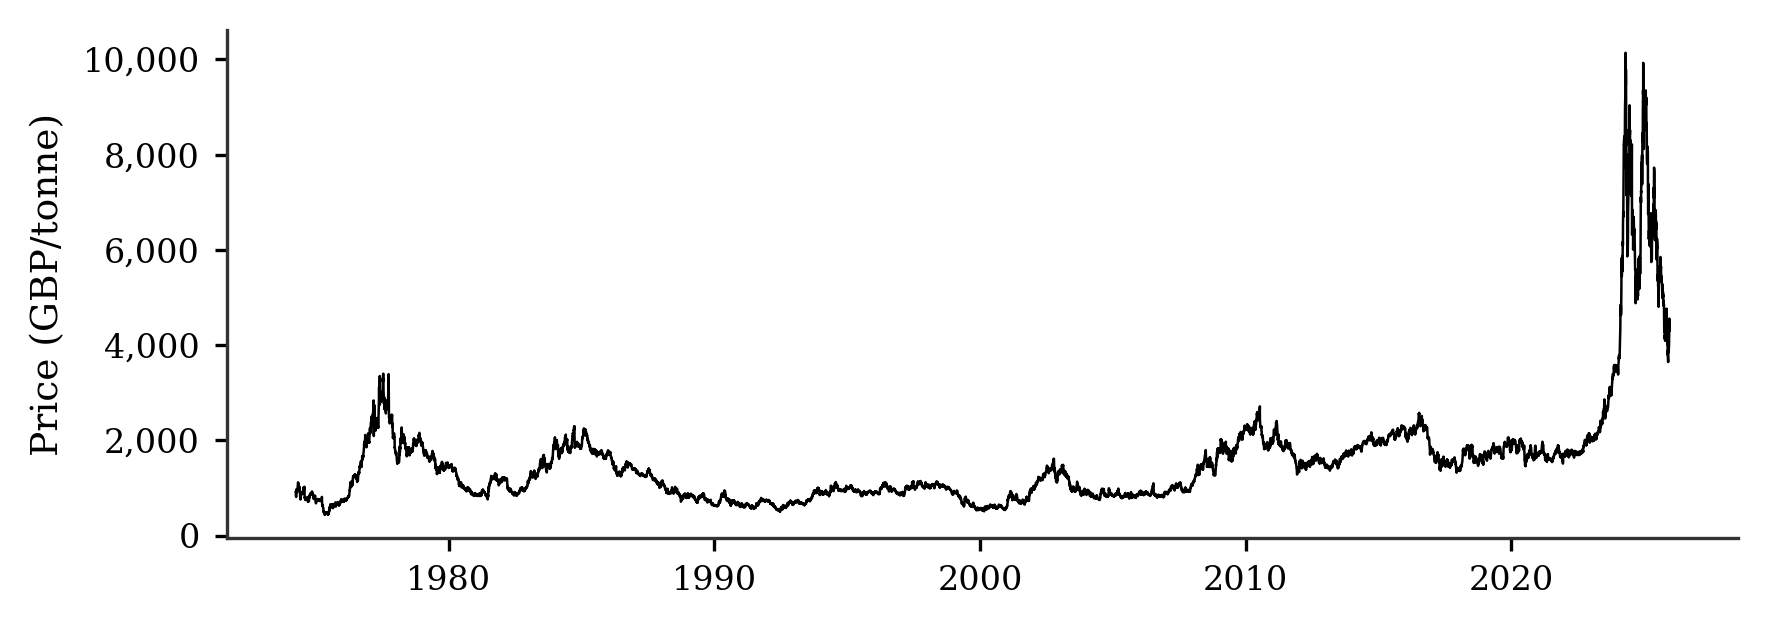
\includegraphics[width=\textwidth]{figures/price_series.png}
\caption{ICE London Cocoa Futures Daily Closing Price (1974--2025)}
\label{fig:price-series}
\begin{tablenotes}
\small
\item \textit{Notes}: Front-month continuous contract (LCCc1) daily closing
prices in GBP per metric tonne. Data source: Refinitiv Workspace.
Sample period: April 1, 1974 -- December 15, 2025 (13,090 trading days).
\end{tablenotes}
\end{figure}

Table~\ref{tab:return-stats} presents descriptive statistics for daily
log-returns. The mean daily return is slightly positive (0.012\%), corresponding
to an approximate annualized mean return of 3\% over the full sample. However,
returns exhibit substantial volatility: the standard deviation of 1.93\%
implies an annualized volatility of approximately 30\%, consistent with cocoa's
classification as a high-volatility commodity. The distribution of returns
deviates sharply from normality. Negative skewness ($-0.997$) indicates a
left tail longer than the right, reflecting the tendency for large negative
price movements to occur more frequently than large positive ones. Excess
kurtosis of 12.96 documents fat tails: extreme returns occur far more often
than a Gaussian distribution would predict. The Jarque-Bera test decisively
rejects normality ($p < 0.001$), confirming that standard volatility models
assuming Gaussian innovations may be misspecified for cocoa returns.

\begin{table}[htbp]
\centering
\caption{Descriptive Statistics for Daily Log-Returns}
\label{tab:return-stats}
\begin{tabular}{lr}
\toprule
\textbf{Statistic} & \textbf{Value} \\
\midrule
Observations & 13,087 \\
Mean (\%) & 0.012 \\
Median (\%) & 0.000 \\
Std. Deviation (\%) & 1.929 \\
Minimum (\%) & $-26.212$ \\
Maximum (\%) & 12.988 \\
25th Percentile (\%) & $-0.917$ \\
75th Percentile (\%) & 0.945 \\
\addlinespace
Skewness & $-0.997$ \\
Excess Kurtosis & 12.963 \\
\addlinespace
Jarque-Bera & 141,013 \\
\quad $p$-value & $<0.001$ \\
\bottomrule
\end{tabular}
\begin{tablenotes}
\small
\item \textit{Notes}: Daily log-returns computed as $r_t = \ln(C_t / C_{t-1})$ for ICE London cocoa front-month continuous contract (LCCc1), April 1974--December 2025. Returns expressed in percentage points. Excess kurtosis reported (normal distribution: 0). Jarque-Bera test strongly rejects normality ($p < 0.001$), consistent with fat tails and negative skewness typical of commodity returns.
\end{tablenotes}
\end{table}


\paragraph{Volatility time series.}
Figure~\ref{fig:volatility-series} displays the Yang-Zhang volatility
estimator (annualized, in percent) computed from daily OHLC data. The
figure reveals pronounced volatility clustering:
periods of high volatility persist for extended intervals before reverting
to lower levels. The late-1970s episode and the 2022--2024 crisis stand out
as the two dominant volatility regimes in the sample. Between these episodes,
volatility fluctuates around a lower baseline with occasional spikes
corresponding to supply shocks, weather events, and financial market
turbulence (e.g., the 2008 financial crisis).

\begin{figure}[htbp]
\centering
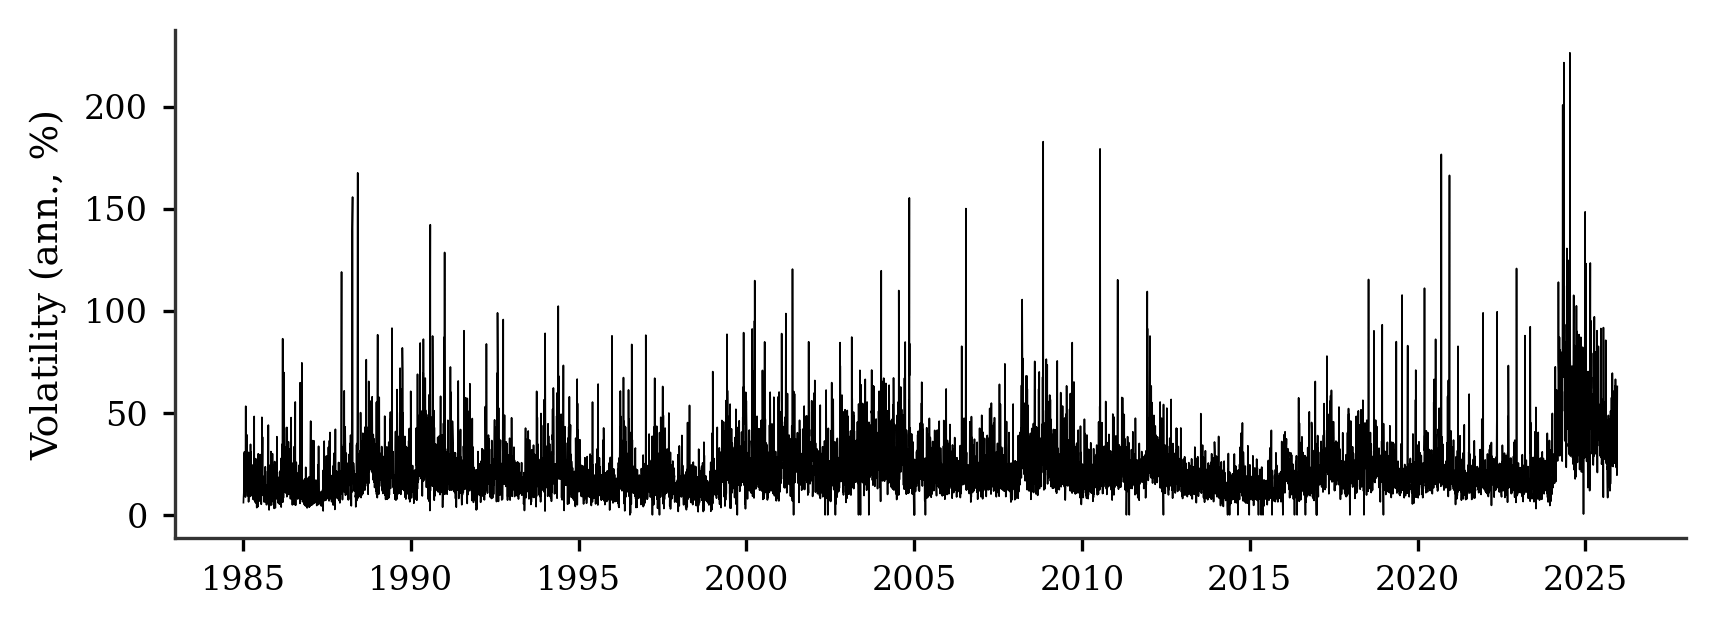
\includegraphics[width=\textwidth]{figures/volatility_timeseries.png}
\caption{Yang-Zhang Annualized Volatility Time Series (1974--2025)}
\label{fig:volatility-series}
\begin{tablenotes}
\small
\item \textit{Notes}: Yang-Zhang volatility estimator computed from daily
OHLC prices and annualized (percent). The estimator combines overnight,
intraday, and close-to-close variance components following
\textcite{yangDriftIndependentVolatility2000}. Pronounced volatility clustering
and regime-switching are evident, motivating the use of HAR models that
capture persistence across multiple horizons.
\end{tablenotes}
\end{figure}

The persistence of volatility justifies the HAR model's multi-horizon
structure: current volatility depends not only on yesterday's volatility
(daily component) but also on average volatility over the past week and
month (weekly and monthly components). The clustering pattern also motivates
quantile regression: during high-volatility regimes, the tails of the
volatility distribution shift outward, and point forecasts of the mean may
underestimate the risk of extreme outcomes.

\paragraph{Stationarity.}
The regression models in Section~\ref{sec:methodology} require stationary
inputs. Table~\ref{tab:stationarity} reports Augmented Dickey--Fuller (ADF)
and Phillips--Perron (PP) unit root tests for the three key series. Both
tests include a constant; ADF lag length is selected by AIC.

\begin{table}[htbp]
\centering
\small
\caption{Unit root tests for stationarity}
\label{tab:stationarity}
\begin{tabular}{lrccrcc}
\toprule
 & & \multicolumn{2}{c}{ADF} & & \multicolumn{2}{c}{PP} \\
\cmidrule(lr){3-4}\cmidrule(lr){6-7}
Series & $N$ & Statistic & $p$-value & & Statistic & $p$-value \\
\midrule
Log returns & 13,087 & $-112.08$ & $<0.001$ & & $-112.09$ & $<0.001$ \\
Yang-Zhang volatility & 13,087 & $-8.42$ & $<0.001$ & & $-90.99$ & $<0.001$ \\
Ni\~no 3.4 anomaly & 787 & $-6.85$ & $<0.001$ & & $-6.46$ & $<0.001$ \\
\bottomrule
\end{tabular}
\par\smallskip
{\footnotesize\textit{Note:} ADF = Augmented Dickey--Fuller test
\parencite{dickey1979distribution}; PP = Phillips--Perron test
\parencite{phillips1988testing}. Both tests include a constant.
ADF lag length selected by AIC. The null hypothesis is a unit root;
rejection indicates stationarity.}
\end{table}

All three series decisively reject the unit root null at the 1\% level.
Log returns are stationary by construction, with ADF and PP statistics
both below $-112$. The Yang-Zhang volatility series exhibits high
persistence---the ADF test requires 39 lags to whiten the residuals---but
remains stationary (ADF $= -8.42$, $p < 0.001$). The large discrepancy
between the ADF and PP statistics ($-8.42$ vs.\ $-90.99$) reflects the
difference in how each test handles serial correlation: ADF augments the
regression with lagged differences, while PP applies a non-parametric
correction to the test statistic. Both agree on rejection. The Ni\~no~3.4
anomaly is stationary by design, as it measures deviations from a
climatological mean, confirmed by both tests (ADF $= -6.85$, PP $= -6.46$,
$p < 0.001$). These results justify the use of standard OLS and quantile
regression methods without differencing or cointegration corrections.

%------------------------------------------------------------------------------

The data described in this section provide the foundation for the empirical
analysis. The extended daily sample (1974--2025) ensures sufficient variation
in both volatility regimes and ENSO phases, while the availability of
intraday data for the recent period enables validation of the Yang-Zhang
volatility proxy. The next section presents the empirical results from the
HAR-based quantile regression models estimated using these data.
